\documentclass[tikz,border=4pt]{standalone}
\usepackage{amsmath}
\usetikzlibrary{arrows.meta,positioning}
\begin{document}
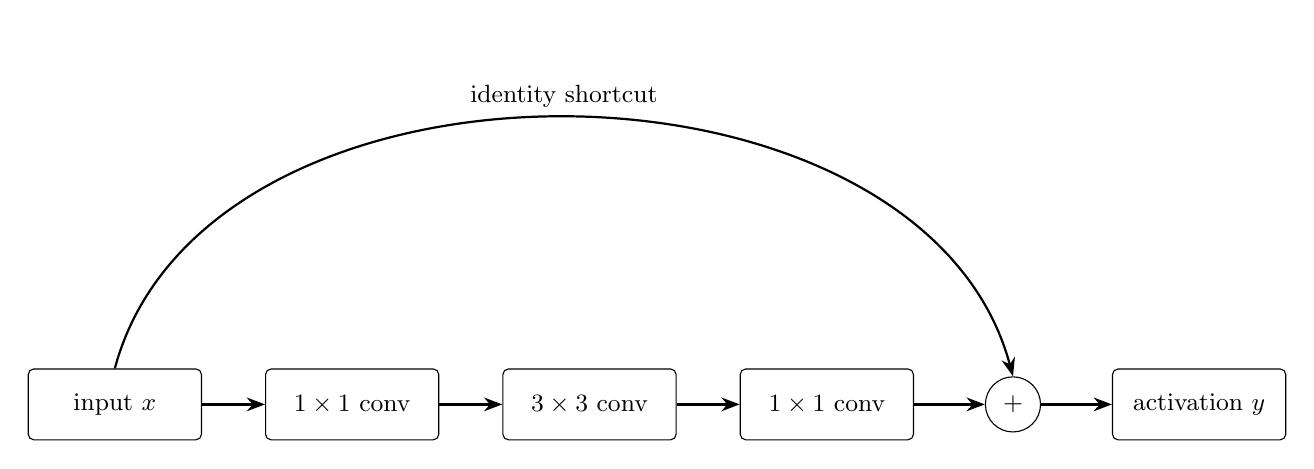
\begin{tikzpicture}[
  >=Stealth,
  node distance=8mm,
  every node/.style={font=\small},
  block/.style={draw,rounded corners=2pt,minimum width=22mm,minimum height=9mm,align=center},
  arrow/.style={->,thick}
]
  \node[block] (input) {input $x$};
  \node[block,right=of input] (conv1) {$1\times1$ conv};
  \node[block,right=of conv1] (conv3) {$3\times3$ conv};
  \node[block,right=of conv3] (conv2) {$1\times1$ conv};
  \node[draw,circle,right=9mm of conv2,minimum size=7mm] (add) {$+$};
  \node[block,right=9mm of add] (output) {activation $y$};
  \draw[arrow] (input) -- (conv1);
  \draw[arrow] (conv1) -- (conv3);
  \draw[arrow] (conv3) -- (conv2);
  \draw[arrow] (conv2) -- (add);
  \draw[arrow] (add) -- (output);
  \draw[arrow] (input.north) to[out=75,in=105]
    node[midway,above] {identity shortcut} (add.north);
\end{tikzpicture}
\end{document}
